%!TEX root = ../dissertation.tex

\chapter{Background}
\label{chapter:background}
In order to develop a programming environment for \gls{gd} that works in the cloud, we first need to study the current solutions.

Not all presented solutions are used exclusively for \gls{gd}.
\gls{gd} encompasses both 3D modeling and programming, so it makes sense to look at systems where at least one of these aspects is explored.
Furthermore, the solutions that are presented include both desktop-based and cloud-based applications to allow for an understanding of what is currently possible in the cloud and how it compares to what is available on the desktop.

For each of the application that will be described, we have to state clearly its nature, that is:
\begin{itemize}
	\item Is it a desktop-based or cloud-based application?
	\item Is it a programming environment? If so, what is its target audience?
\end{itemize}

{\bf(Criteria for what makes a related work.)}

%##############################################################################
%##############################################################################
\section{Related Work}


\subsection{Impromptu}
\label{section:impromptu:related}
Impromptu\cite{sorensen2005impromptu,sorensen2010programming} is a programming environment developed to explore manipulation of musical structure in live performance; an \gls{ide} for musicians and sound artists.

%What is live-performance?
Using Impromptu, live performance takes place as a musician programs algorithms that produce music in front of an audience.
During his performance, the artist writes the program that produces the sounds and chooses the right moments to change it to move between different parts of the music.

%What does it provide to support live-performance?
To enable live programming, Impromptu brings together four components, as stated in \cite{sorensen2005impromptu}: an audio synthesizer, a real-time scheduling engine, a Scheme interpreter and an \gls{ide}.
The first three components make up the runtime environment, responsible for producing the sound, while the last provides an user interface, where the musician writes code and sends it to the runtime in much the same way as using a \gls{repl}.

%Describe live programming experience of impromptu.
As he sends code, the musician builds the algorithm that produces the music incrementally.%
\footnote{The code sent to the runtime can define/redefine functions or variables, and schedule audio or functions to be played or run later.}
To be able to keep producing sound for the audience he can program simple patterns, send them to the runtime and then change them as he programs more elements to compose the music.
As he adds more elements, he can start to make small changes to some of them which will be immediately audible.

The immediacy from program changes to audible ones also lets the musician experiment with new ideas.
Similarly, someone doing \gls{gd} will also benefit from having this immediacy in his \gls{ide}.

The separation of components referred earlier also allows several musicians to collaborate at the same time in a performance\cite{sorensen2005impromptu}.
With their computers connected to the same runtime environment, they can build different parts of the music or, more interestingly, make changes to parts of the other's work.
This is also an interesting aspect to explore in architecture, where several architects can work on a \gls{gd} program at the same time, each one showing his ideas on how to evolve the design.

There is, however, a major difference between composing music and architecture.
As sound is an ephemeral phenomenon, music's complexity comes from how sounds are organized in time as opposed to architecture's complexity, which comes from how shapes are organized in space.
The point is, music/sound generation is a continuous process whilst architecture/form generation is a instantaneous process.
\begin{description}
	\item[Music] produce samples at 44kHz
	\item[Architecture] produce model of 100k shapes + display model of 100k shapes at 25+Hz
\end{description}
There are differences in performance that will affect the architecture of the system and its usage experience.

Impromptu is in the process of being replaced by Extempore\footnote{http://extempore.moso.com.au/}.
Instead of having its own editor, Extempore has plug-ins for several popular code editors.
Extempore also includes a second programming language for programming \glspl{dsp}, which have stricter real-time constraints.



\subsection{LightTable}
\label{lighttable:related}
LightTable\cite{lighttable2015site} is a code editor for the Clojure programming language\cite{hickey2008clojure} and is an example of a desktop application that uses web technologies.
More specifically, it uses nw.js\footnote{http://nwjs.io} as its runtime allowing it to use the html layout engine for its user interface, to use Javascript as its programming language and to use node.js\cite{tilkov2010node} modules.
LightTable is written in ClojureScript\cite{10.1109/MIC.2011.148}, a subset of Clojure that compiles to Javascript.

Although not related to \gls{gd}, LightTable as proposed some interesting features and concepts for \glspl{ide}.

%Why is LightTable relevant?
One of these is the use of the drafting table as metaphor.%
\footnote{http://www.chris-granger.com/2012/04/12/light-table-a-new-ide-concept/}
The metaphor comes from looking at the way work is done in other fields of engineering, where engineers spread all materials relevant to their work over large tables, from tools to reference information.
Instead of displaying the contents of entire files, LightTable divides the code into meaningful units and displays them as small editors spread over the table's surface.
In one of its experimental versions, LightTable also supported displaying running programs in the table.
Figure \ref{fig:lt:draft:table} shows an example of this metaphor, which has some resemblance to node-based/visual programming environments since the programmer still has to think of how to arrange what is on the table.
%What makes it different is allowing to choose what is on the table instead of having everything on it all the time.

\begin{figure}
  \centering
  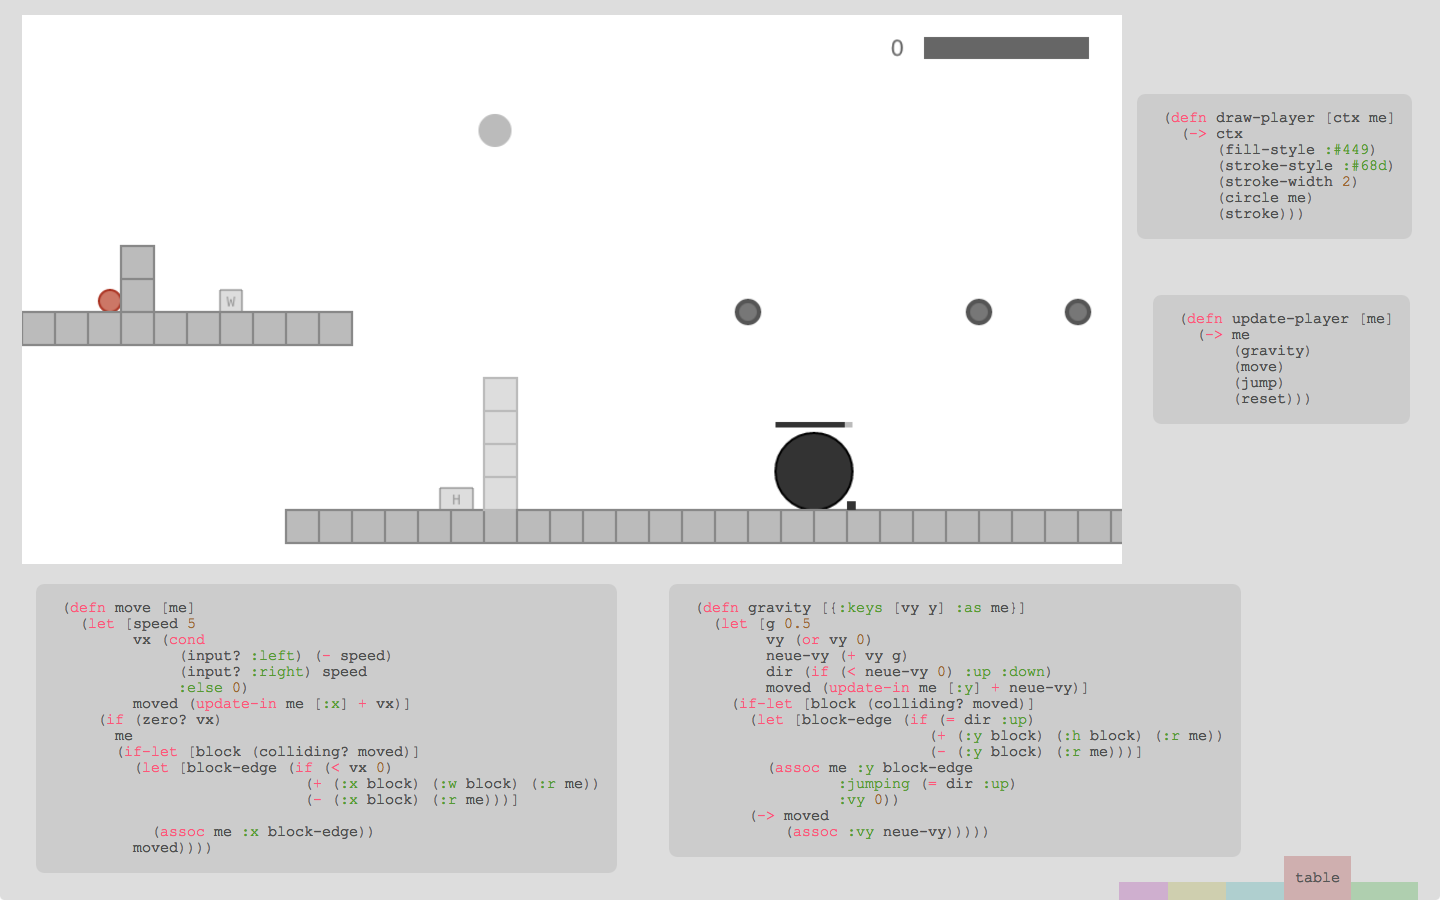
\includegraphics[width=12cm]{./images/lt_game_example__inv}
  \caption[LightTable's drafting table showing a game.]{LightTable's drafting table. A game is being run inside it while some of its code is displayed in separate editors.}
  \label{fig:lt:draft:table}
\end{figure}

%LightTable "function navigation"
Other feature deals with how to help navigating Clojure code bases.
In Clojure, functions are defined inside namespaces and all Clojure definitions (functions, variables, macros) are stored in text files.
Navigating among definitions and the current namespace structure should not get in the way of editing code.
To make editing easier, LightTable provides a \emph{namespace browser} that allows to find functions and a \emph{code document} where functions can be added for editing without moving them out of their namespace or displaying entire files where they are defined.
Figure \ref{fig:lt:clojure:table} shows an experiment where these two are used.

\begin{figure}
  \centering
  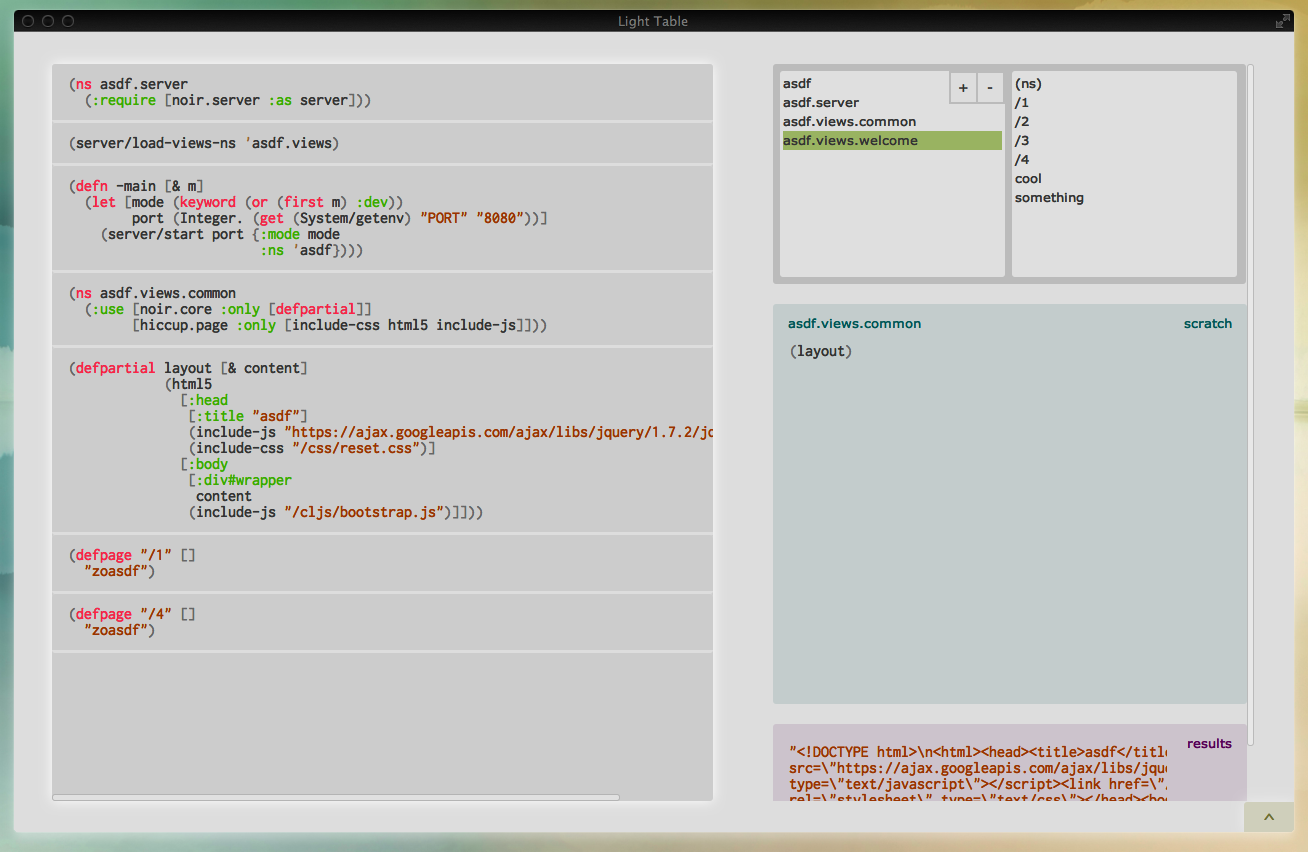
\includegraphics[width=12cm]{./images/lt_clojure_table__inv}
  \caption{An experiment showing a \emph{code document} on the left and a \emph{namespace browser} on the top right.}
  \label{fig:lt:clojure:table}
\end{figure}

%LightTable "variable substitution"
Another interesting feature of LightTable is its ability to show data flow in a function call.
Since the main purpose of a function is to transform its input data into its output data, it helps to see what happens to the data on each step of the function.
To achieve this, LightTable overlays variable values and return values, respectively, on each variable occurrence and expression of the function.
Figure \ref{fig:lt:val:overlay} shows an example of such functionality.
This functionality is part of LightTable's \emph{instarepl}.

This last feature has the problem of not being capable of showing the data-flow for more than one run of a part of the code.
If a function is called more than once then it will be more useful to show the data-flow of all the calls.

\begin{figure}
	\centering
	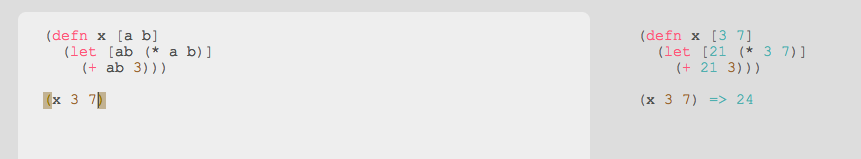
\includegraphics[width=12cm]{./images/lt_val_overlay__inv}
	\caption{An example of LightTable's value overlaying. The occurrences of the variables \emph{a}, \emph{b} and \emph{ab} were replaced with their values while evaluating the expression \emph{(x 3 7)}; the result of this expression is also overlaid.}
	\label{fig:lt:val:overlay}
\end{figure}

Finally, the way LightTable is structured is also relevant as it makes possible to modify its behavior at runtime.
The main design pattern used in LightTable is the \gls{bot} pattern.
As described by one of its developers,\footnote{http://www.chris-granger.com/2013/01/24/the-ide-as-data/ at Nov/2015.} LightTable can be described as a set of \emph{Objects}, each having a set of \emph{Behaviors} and being tagged with a set of \emph{Tags}.
The \emph{Behaviors} describe how an \emph{Object} reacts when events are raised on it. \emph{Tags} are groups of \emph{Behaviors}.
When an event is raised on an \emph{Object} both its \emph{Behaviors} and those from its \emph{Tags} are notified.


\subsection{IPython}
\label{section:ipython:related}
IPython\cite{PER-GRA:2007} is a programming environment (Figure \ref{fig:ipython:notebook}) directed towards providing better, more straightforward, scientific computing.

%Why is it important? I cannot imagine designers using it.
IPython can be used as a command shell by using its notebook \gls{ui}, the IPython notebook.
As seen in Figure~\ref{fig:ipython:notebook}, IPython's notebooks can contain not only source code but also results and rich text.
The notebooks are displayed using an interactive web page.

The style of producing notebooks in IPython is one that mixes programming, writing and exploring.
Interestingly, this style is also part of a designer's processes.
Like a scientist, the designer also has to do exploration of ideas (design ideas in his case), reach conclusions (finished designs) and share his work with others (fellow designers, clients, friends, blog readers).
Unfortunately, although IPython notebooks are natural tools for exploration, they do not provide domain specific functionality for architecture.

As its name suggests, IPython's main programming language is Python.
Nevertheless, other popular programming languages can be used in IPython, particularly those popular in the scientific community like R, or Julia.%
\footnote{More language kernels can be found in IPython's github page: https://github.com/ipython/ipython/wiki/IPython-kernels-for-other-languages}

One trend in its community, one that is supported by IPython notebooks, is to make results in publications more reproducible.
Typically, the code used to compute the results showed in publications is not made available to the public, so it is harder for a stranger to check them.
Instead of publishing a PDF or making a blog post, authors write whole publications as IPython notebooks which then are shared and thus allow everyone to run their source code.
Having access to a working copy of the notebook, one can also experiment with it to better understand it, form own conclusions, and find potential errors.

%IPython architecture
To allow more flexibility between the core computing functionality and the \gls{ui}, IPython was decomposed into execution kernels, a communication protocol, and several front-ends.
Execution kernels are responsible for running the code of notebooks and front-ends implement the \gls{ui}, as is the case of IPython's notebooks.
The communication protocol defines how communication between execution kernels and front-ends is done.
With this, it is possible to implement new execution kernels for running code from a programming language not yet implemented or an alternative front-end different from IPython notebooks.
Moreover, the communication protocol also allows execution kernels and front-ends to run on different computers\cite{PER-GRA:2007}.

IPython has given rise to the Jupyter project\footnote{https://jupyter.org/}, which aims to make IPython's model of interaction ready for the cloud.
In the context of Jupyter, IPython is now only concerned with providing an interactive Python experience.

\begin{figure}
	\centering
	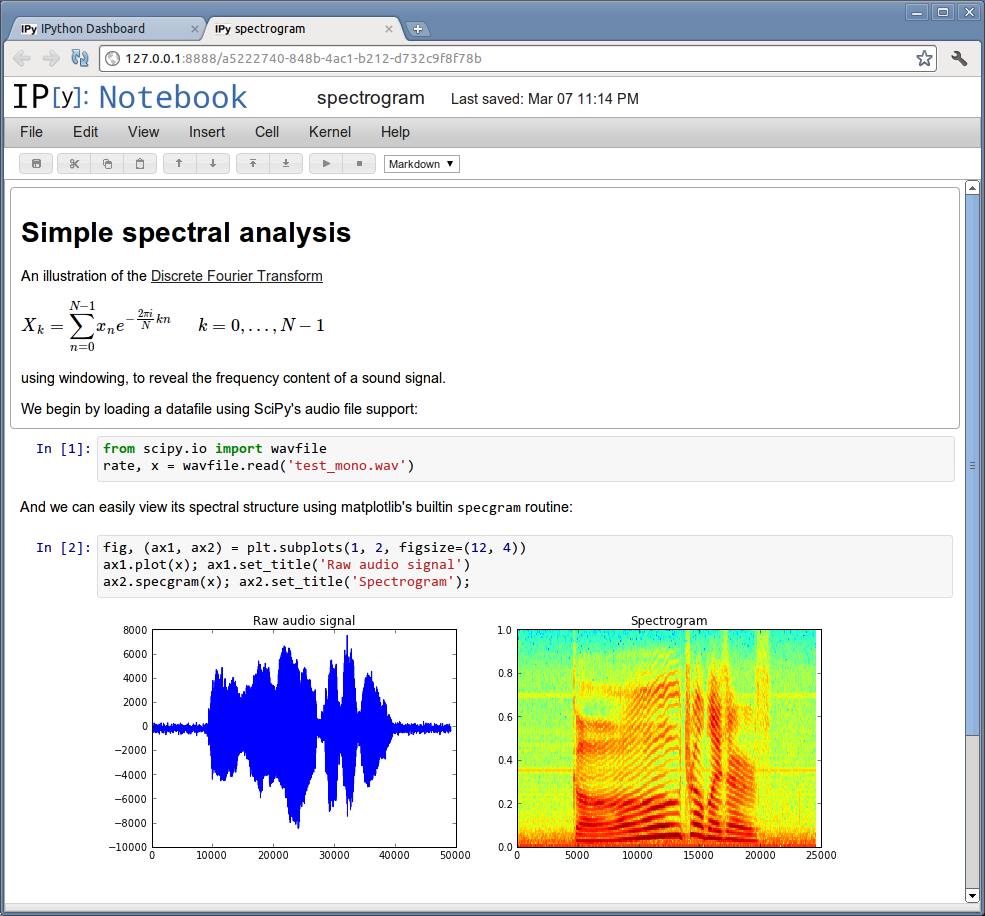
\includegraphics[width=0.8\textwidth]{images/ipython_notebook}
	\caption{An IPython notebook with rich text, mathematical notation, source code and results from executing such code.}
	\label{fig:ipython:notebook}
\end{figure}


\subsection{OpenJSCAD}
OpenJSCAD\cite{openjscad2015site} is a project aiming to implement OpenSCAD\cite{kintel2011openscad} using web technologies.
Instead of using OpenSCAD's language, OpenJSCAD uses JavaScript as its language.
Most of OpenSCAD functionality is implemented in OpenJSCAD.
Like OpenSCAD, it focuses on creating 3D models for 3D printing.

Similarly to the \gls{gd} approach, to actually model in OpenJSCAD the user has to write a program in either JavaScript or OpenSCAD's language.

Being an environment for modeling 3D printed objects, OpenJSCAD supports importing and exporting 3D models from/to STL and AMF files which are commonly used as 3D printing formats.

OpenJSCAD provides two user interfaces, one \acrfull{cli} and one \acrfull{gui}, the latter implemented as a web page.%
\footnote{https://github.com/Spiritdude/OpenJSCAD.org}
Moreover, the first can be used for batch processing, while the second integrates an editor to edit a program and a 3D view for viewing the corresponding results.
This separation enables the use of OpenJSCAD for programming without requiring the programmer to install anything more than a web browser, which is almost always already installed.
This is just a matter of convenience, since both interfaces perform the same work to generate the models and both can export them as files.

OpenJSCAD makes its functionality available as functions as well as methods on its objects, which makes writing programs more flexible.
This way, one can write either \mintinline{javascript}{a.union(b).translate([1,0,3])}, \mintinline{javascript}{translate(union(a,b), [1,0,3])} or \mintinline{javascript}{union(a,b).translate([1,0,3])} depending on what is more readable.%
\footnote{The first can be read as \emph{a united with b, translated by [1,0,3]}, the second as \emph{the translation of the union of a and b by [1,0,3]} and the third as \emph{the union of a and b, translated by [1,0,3]}.}

Both OpenJSCAD's functions and methods return new objects and do not have side-effects.
This allows the programmer to use the functional programming paradigm and makes it easier to understand programs, as there are less side-effects that could change their behavior.

A problem that can arise while writing and testing JSCAD programs is that there is no help on getting the parameters for operations right and it is frustrating to spend more time than acceptable trying to understand why a certain operation is not producing the desired result.
This problem is even more relevant when most of the operations have multiple optional parameters and there are parameters that replace other parameters.
Currently, the only help available is OpenJSCAD's documentation (a tour on its functionality), the online community around OpenJSCAD and, since Javascript is its language, web browsers' Javascript developer tools.


\subsection{Processing}
\label{section:processing:related}
Processing\cite{reas2007processing} is a programming language and a development environment aimed at ``promoting software literacy in the visual arts and visual literacy within technology''.%
\footnote{Quoting https://www.processing.org, 9/Nov/2015.}
It is a desktop application.

Processing enables everyone to write programs that both draw to the screen and react to input from the user, like moving the mouse or pressing a key on the keyboard.
It makes this possible by implementing most of the functionality that is commonly required, like initializing the drawing surface, so the programmer only has to implement the functionality specific to the result he wants to achieve.
The code in Listing \ref{lst:simple:processing}, for instance, is what is needed to setup a drawing canvas, its background color and continuously draw a line from the mouse position to a point on the canvas.

To use Processing's programming language, one needs to use its \gls{ide}, the \acrfull{pde}.
As shown in Figure \ref{fig:proc:dev:env}, the \gls{pde} includes a text editor with syntax highlighting and runs Processing programs.

\begin{listing}
\begin{minted}[linenos,frame=lines]{java}
//Hello mouse.
void setup() {
	size(400, 400);
	stroke(255);
	background(192, 64, 0);
}

void draw() {
	line(150, 25, mouseX, mouseY);
}
\end{minted}
	\caption[A simple Processing sketch]{A simple Processing sketch}
	\label{lst:simple:processing}
\end{listing}

\begin{figure}
	\centering
	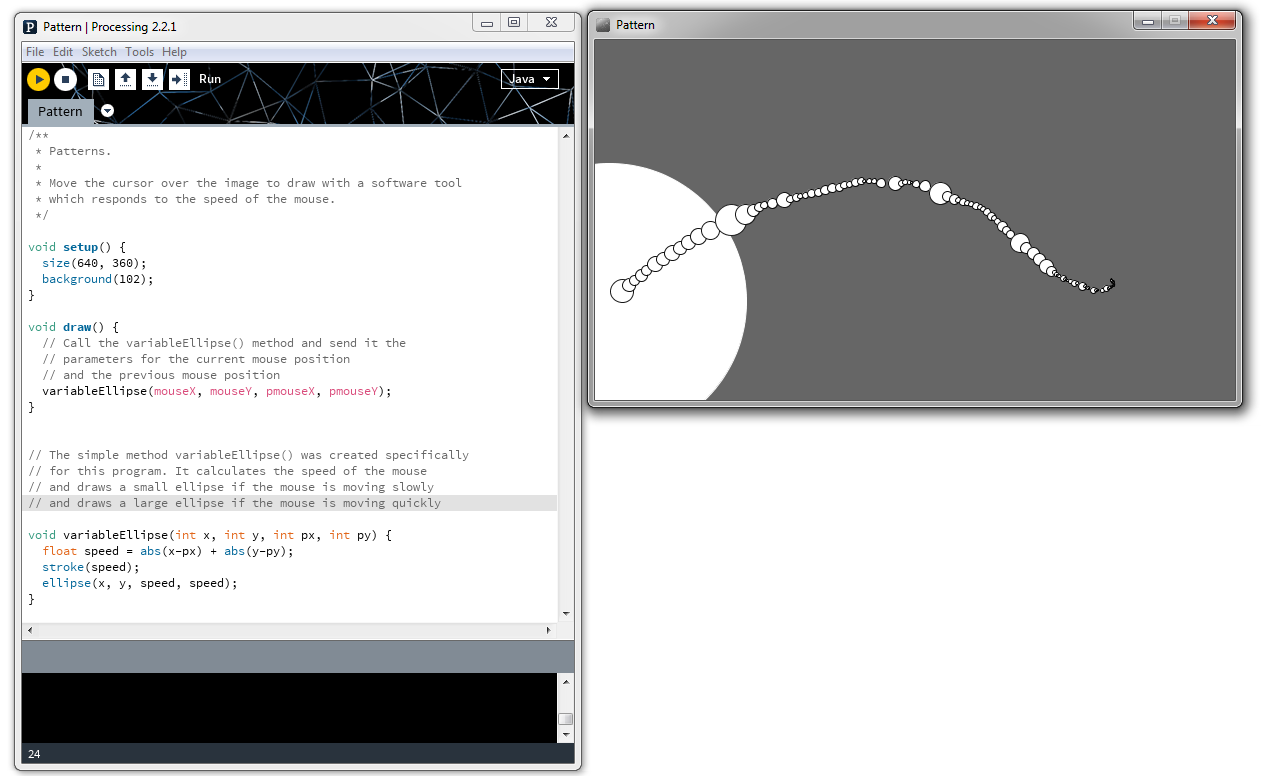
\includegraphics[width=1.0\textwidth]{images/proc_dev_env}
	\caption{On the left: The \gls{pde} displaying an example \emph{sketch} while it is being run. On the right: The drawing window to which the \emph{sketch's} instructions are applied.}
	\label{fig:proc:dev:env}
\end{figure}

Processing is sometimes used by architects for exploring design ideas.
However, since most of its functionality revolves around graphics for the visual arts, its use is normally restricted to 2D designs and cannot be used as a full-fledged tool for \gls{gd}.

Several projects have stemmed from Processing to extend its functionality to different programming languages.
These include Processing.py\footnote{http://py.processing.org/}, that extends the \gls{pde} to support Python, and p5.js\footnote{http://p5js.org/}, that provides JavaScript libraries to create interactive web pages.


\subsection{DesignScript}
\label{section:designscript:related}
DesignScript\cite{aish2012designscript} is a programming language that was designed to suit the needs of architecture related design.

%DesignScript programming paradigms
DesignScript uses concepts from multiple programming paradigms like object-oriented, functional and associative programming.
Entities have properties that can be either data or functions like in object-oriented languages; functions' most important role is to take some input and produce some output without producing side-effects like in functional languages; and dependencies among variables are retained like in associative languages.

It supports both imperative (following instructions step-by-step) and associative (propagating changes in a dependency graph) control flows.
The programmer can choose to have portions of the code following one type of control flow and other portions following the other.

%DesignScript primitives
Being a domain-specific language for architecture, DesignScript provides functions for 3D modeling such as creating concrete 3D objects, like cubes and spheres, as well as abstract geometry, like planes and points, that is used as scaffolding.

DesignScript also supports lists of values and lets them be used in place of single parameters in calls to functions.
This lets architects use lists more easily as they do not have to use loops to extract values and pass them to functions.%
\footnote{If only one of its parameters is receiving a list instead of a value, the function is called once with each value on the list.
If more than one parameter is receiving a list, the function is called with the values combined by either a cross product or a zip of the lists.}

Having modeling primitives and combining several programming paradigms allows the architect to draw from knowledge about architecture modeling while empowering him to express the processes in which those primitives are used.

%DesignScript editor(s)
Editing DesignScript programs can be done either by writing or by creating a graph.
The graph representation is a more natural visualization of the dependencies between the variables of a program when the associative paradigm is being used.
Function calls and variables are represented by nodes, drawn as boxes with slots, that can be connected by wires, which in turn represent data dependencies between nodes.
The written representation of DesignScript is a sequence of statements that specify the relationship between a variable and other variables; defining functions, using the imperative paradigm and reassigning variables is also possible.

DesignScript is used in several environments, all of which are desktop applications.
These include a textual editor in Autodesk AutoCAD (Figure \ref{fig:ds:autocad}), a dedicated graph editor called DesignScript Studio (Figure \ref{fig:ds:dsstudio}) and Dynamo (Figure \ref{fig:ds:dynamo}), which integrates with Autodesk Revit.
Both DesignScript Studio and Dynamo use graph based program editing.

\begin{figure}
	\centering
	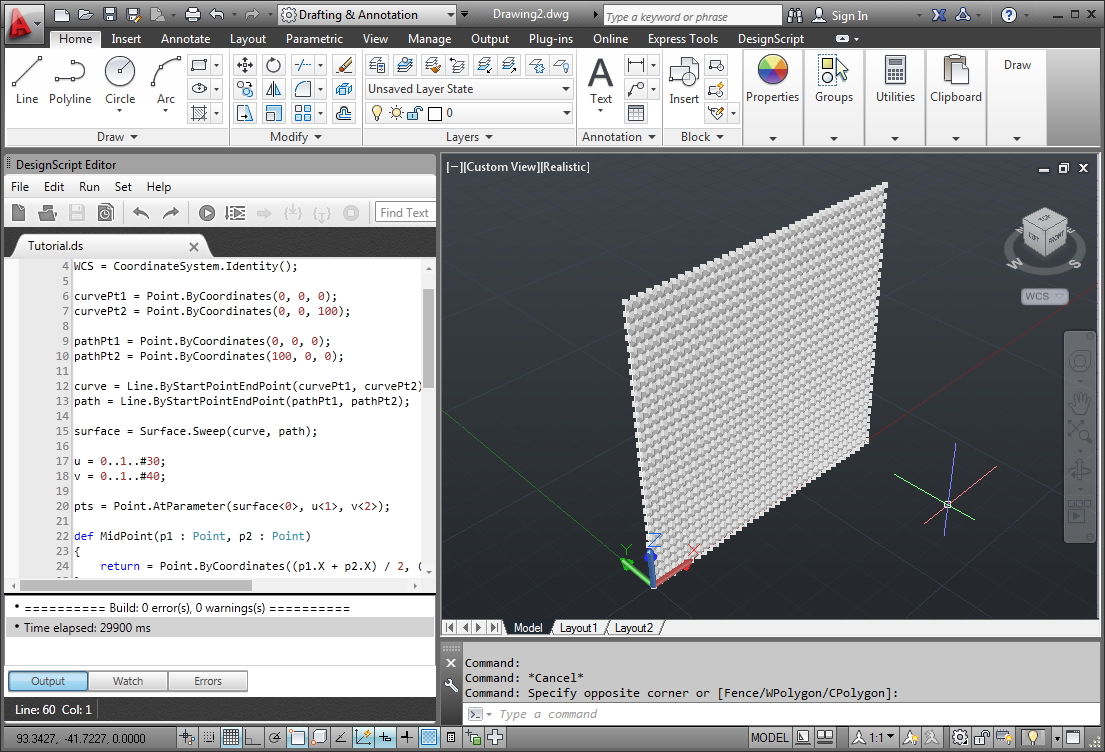
\includegraphics[width=0.8\textwidth]{images/ds_autocad}
	\caption[A DesignScript program being edited in a special text editor inside AutoCAD.]{A DesignScript program being edited in a special text editor inside AutoCAD. This text editor provides auto-complete and a debugger.}
	\label{fig:ds:autocad}
\end{figure}

\begin{figure}
	\centering
	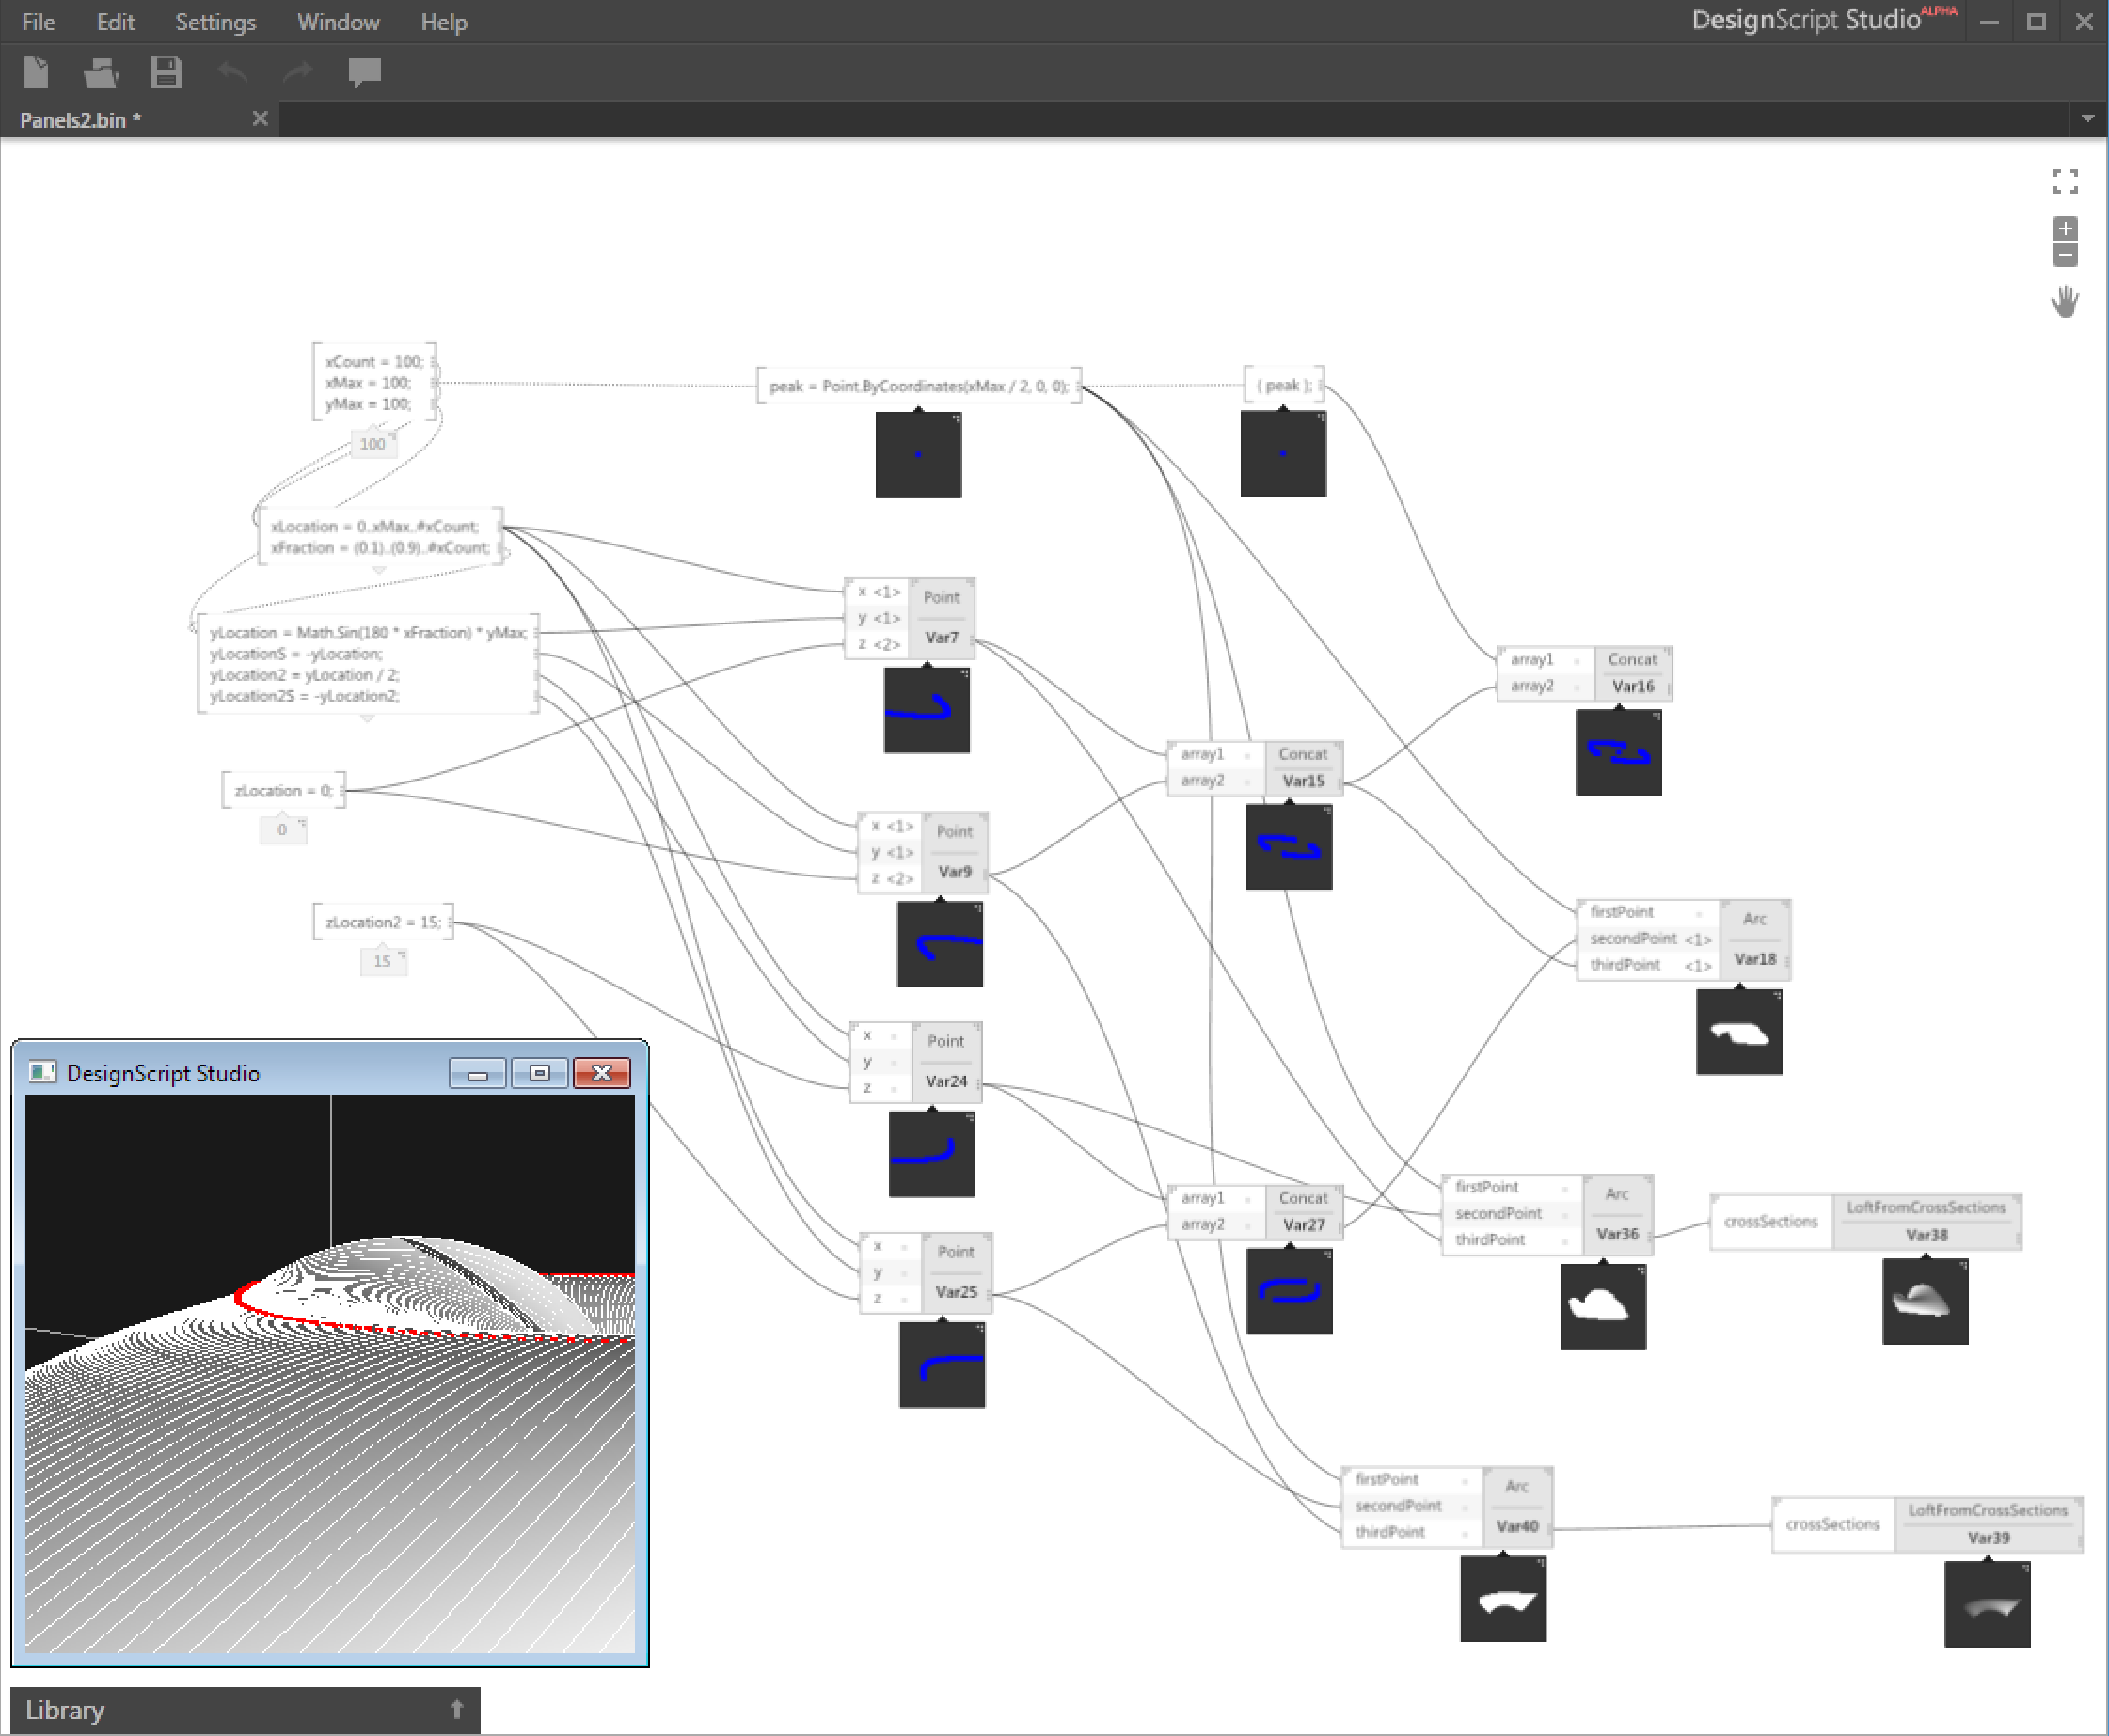
\includegraphics[width=0.8\textwidth]{images/ds_dsstudio}
	\caption[A DesignScript program as a graph in DesignScript Studio.]{A DesignScript program as a graph in DesignScript Studio. Each node can display a preview of its results. To the bottom left corner is a preview of the whole program results and a folded library tab. The library tab contains everything that can be used in the program.}
	\label{fig:ds:dsstudio}
\end{figure}

\begin{figure}
	\centering
	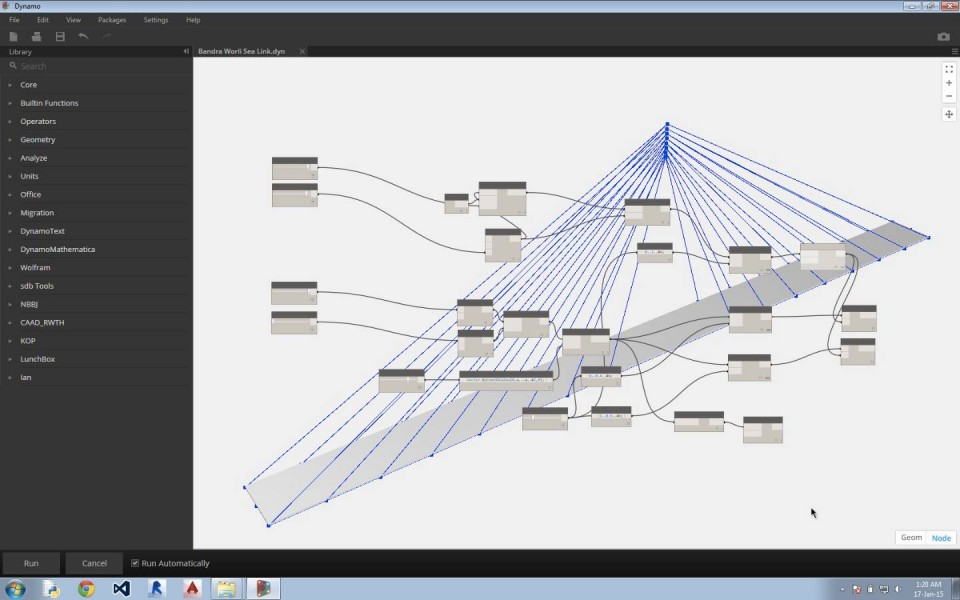
\includegraphics[width=0.8\textwidth]{images/ds_dynamo}
	\caption[Another DesignScript program as a graph in Dynamo. Like in DesignScript Studio, a preview of the result of the program is displayed.]{Another DesignScript program as a graph in Dynamo. Like in DesignScript Studio, a preview of the result of the program is displayed. A difference is that there is only one preview ``canvas''; the preview from selected nodes is highlighted.}
	\label{fig:ds:dynamo}
\end{figure}

Debugging DesignScript programs depends on the environment being used.
The textual environment allows following the execution of the program step-by-step while also supporting watches and breakpoints.
The graph-based environments allow highlighting and listing results of each node.
Both the textual and the graph-based environments provide a preview of the execution of programs.


\subsection{Rosetta}
\label{section:rosetta:related}
Rosetta\cite{de2012modern,lopes2011portable}, shown in Figure \ref{fig:rosetta:ex}, is an environment for \gls{gd}.

Most \glspl{cad} architects use allow them to make \gls{gd} programs.
Unfortunately, as each of these CADs has specific primitive operations, programs written for one CAD will only work in that CAD.
A phenomenon called vendor lock-in.
As an example, if the architect writes a program for AutoCAD, he cannot use it in Rhinoceros3D.
As a result, if he really wants to use it in Rhinoceros3D, he has to rewrite the program taking into account the differences between primitive operations of both \glspl{cad}.

Rosetta's motivation is to allow architects to write portable \gls{gd} programs that generate equivalent models in any CADs they use.
Rosetta allows the architect to choose the front-end programming language and the back-end where the primitive operations will be performed\cite{de2012modern}.%
\footnote{Some front-ends supported by Rosetta are AutoLisp (one of AutoCAD's programming languages), Javascript, Racket and Python; some of the supported back-ends include CADs like Autodesk AutoCAD, Autodesk Revit, Sketchup, and Rhinoceros 3D and also graphics libraries like TikZ and OpenGL.}
This way, the architect can experiment with \gls{gd} without having to switch \gls{cad} and he can also share programs with others using different \glspl{cad}.

Additionally, Rosetta also allows programs written in one programming language to use not only parts from programs written in the same language, but also from programs written in other languages.
This makes it possible for architects to share programs written in different programming languages and also allows them to choose the programming language that best fits each part of the program they are working on.

\begin{figure}
	\centering
	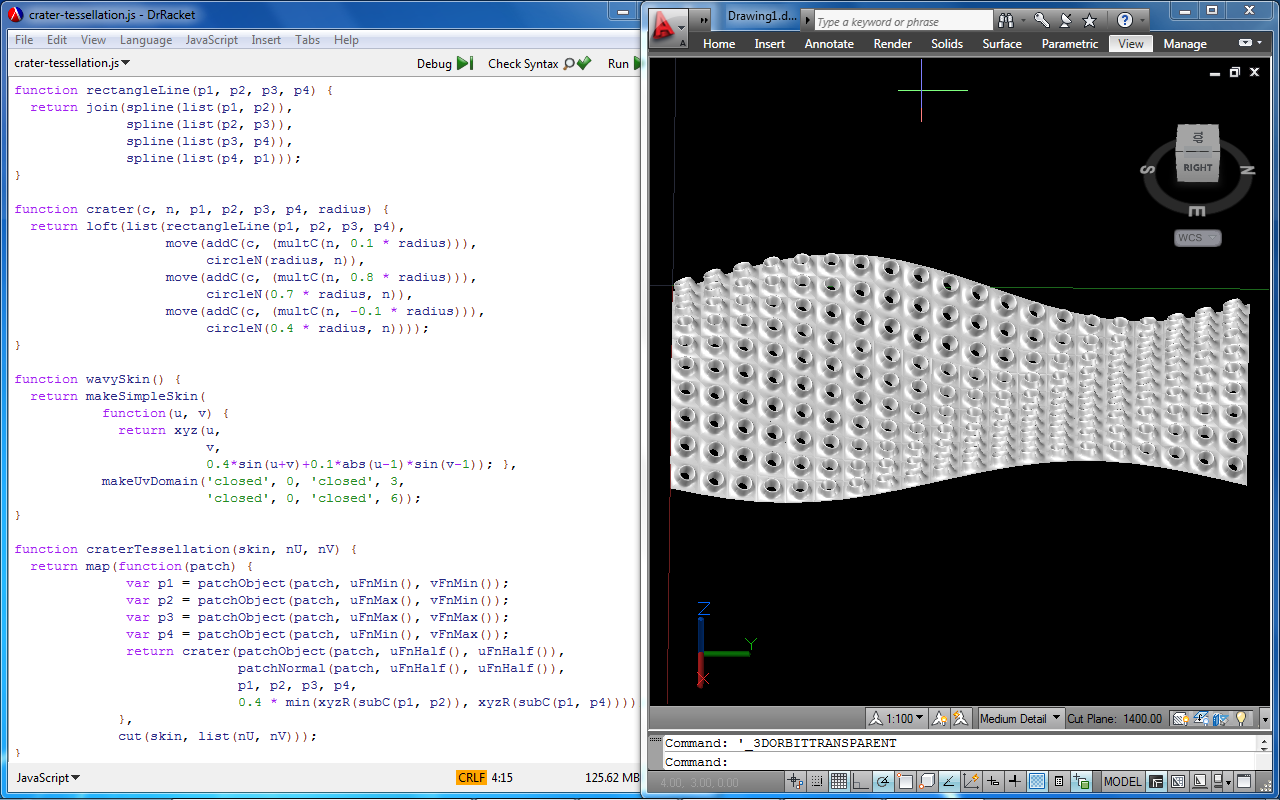
\includegraphics[width=0.8\textwidth]{images/rosetta_js_autocad}
	\caption{A Rosetta program (left) and AutoCAD displaying its results (right). The program is written in Javascript.}
	\label{fig:rosetta:ex}
\end{figure}


\subsection{Clara.io}
Clara.io\footnote{https://clara.io/}\cite{houston2013clara} is a cloud application for 3D modeling and animation, similar to desktop software like Blender and 3ds Max.
Being in this category, Clara.io is more indicated for artistic work as opposed to technical work.
Nonetheless, it can be used in architecture projects to make architectural visualizations.

Using Clara.io closely resembles working with its desktop counterparts.
Modeling is done by adding 3D entities to the scene's scenegraph and afterwards adding modifiers to them and/or directly manipulating them in 3D space(position, rotation, scaling, selection, grouping).

Apart from having features close to other 3D modeling software, being a cloud application Clara.io also supports cloud storage of scenes, real-time collaboration and has integration with VRay cloud rendering.
Furthermore, Clara.io only requires a web browser compatible with HTML5 and WebGL without any installation.
Like so, its users are free to switch between computers without having to configure anything and without having to move their work.

Clara.io's real-time collaboration lets users edit scenes simultaneously.
It gives users an environment where they can work together on tasks that, due to the limitations of files, would have to be performed in isolation to avoid edit conflicts.
For example, they can build a scene simultaneously, each one working on a part, but this time anyone sees the others changes immediately.

When it comes to programming, Clara.io has support for scripting and allows the creation of plug-ins to extend its functionality.%
\footnote{https://clara.io/learn/sdk}
It is possible to use Clara.io's scripting to do \gls{gd}, however, if a user wishes to do so he needs to learn the scene's data model and how to use the scripting \gls{api} to manipulate it, which poses a considerable barrier when compared with existing \gls{gd} environments.


\subsection{OnShape}
OnShape\footnote{https://www.onshape.com/} is a cloud based \gls{cad} application that can be accessed using either a web browser or its mobile app.
As opposed to the systems we talked about earlier, OnShape is a \gls{cad} for mechanical modeling and, as such, its users are familiar with \glspl{cad} like SolidWorks and Autodesk Inventor.
Being a mechanical modeling tool means that the focus is directed towards assembling individual objects instead of buildings, so the working scales are smaller and there is more information on how parts relate to each other.

OnShape has version control of project documents (drawings, 3d models, text documents) and supports real time collaboration.
Like most cloud applications, OnShape promotes collaboration on development teams where team members work remotely.
In order to do this, it allows users to work on the same copy of files as opposed to each working with his own copy, and therefore changes are synchronized automatically.
As users can edit the same copy of a file at the same time, OnShape shows each user what the others are doing to enhance real time collaboration.
It is also possible to create branches of the document when it is necessary to work on different design options or to work on changes in isolation.
Later, changes made in a branch can be merged back into the main branch.

OnShape also includes a dedicated programming language, FeatureScript\footnote{https://www.onshape.com/featurescript}, for defining features for its models.
OnShape includes an \gls{ide} for FeatureScript but the language does not aim to replace OnShape's modeling approach based on interactively manipulation the model's feature list.


\subsection{Mobius}
%Prototype\\
%Parametric modeling? Block based programming + Visual programming? 3D modeling? Higher-order functions? Web application?\\
%Refs: http://mobius.design-automation.net/papers

{\bf(glossary: higher-order function)}\\
Mobius is a visual programming environment for 3D modeling.
It tries to make visual programming environments as powerful as textual programming environments by bringing associative and imperative programming together and by supporting higher-order functions, common in textual programming languages\cite{Janssen2016}.

In Mobius, programs are a combination of nodes in a data-flow graph that ultimately produces a 3D model.
The architect can implement nodes by assembling an imperative procedure out of virtual building blocks, which can be loops, function calls or variable assignments.
This way, Mobius tries to get the best of visual and textual programming languages.

To support higher-order functions, Mobius adds an output to every node that contains the function representing that node.
This way, the node can be passed to other nodes as an input.
Nodes receiving the function can then use it to perhaps generate an element of a grid parameterized by its coordinates or to generate the shape of a balcony.

Finally, Mobius is implemented as a web page and like so is available to any computer connected to the Internet and does not require installation.


%\subsection{RepoCad}
%Prototype\\
%2D drawing? Integrated version control? Sharing library?
%Where is the juice???


\subsection{Antimony}
%Refs: matt keeter thesis(predecessor) + blog\\
%Design to fabrication pipeline?\\
%http://www.mattkeeter.com/projects/antimony/3/

Antimony\footnote{https://github.com/mkeeter/antimony} is a desktop application for solid modeling where models are described by data-flow programs.
Programs are edited using a node-based representation like in visual programming environments.
When editing a program, Antimony also displays handles in the 3D view that can be dragged with the mouse to change free node inputs, as shown in Figure \ref{fig:antimony:handles}.

Antimony was implemented as a tool to be used from design to fabrication, so it can generate files for machining or 3D printing its models.

It is possible to implement custom nodes by writing a Python program with custom directives.
This program defines what are the inputs and outputs of the node and what is its \gls{ui} in the 3D view.
As Antimony uses \glspl{sdf} as its representation of solids, shapes are defined by specifying a formula for the shape's \gls{sdf} and its domain bounds.

\begin{figure}
	\centering
	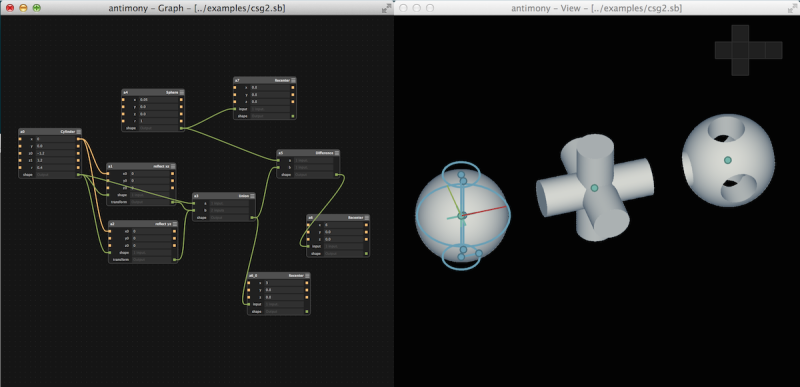
\includegraphics[width=0.8\textwidth]{images/antimony_ui_handles}
	\caption{Antimony allows the user to adjust parameters using handles in the 3D view.}
	\label{fig:antimony:handles}
\end{figure}


%##############################################################################
%##############################################################################
\section{Comparison}


\begin{table}
	\centering
	\renewcommand{\arraystretch}{1.2}

	\begin{tabulary}{\textwidth}{lLL}
		\toprule
		{\bf Environment}	& {\bf Domain} 						& {\bf Programming Purpose}												\\
		\midrule
		Impromptu			& music, live coding			& schedule sound generation + implement \glspl{dsp}	\\
		LightTable		& code editing						& general																					\\
		IPython				& scientific computing		& general																					\\
		OpenJSCAD			& 3D CAD									& generate 2D/3D models														\\
		Processing		& visual arts							& draw, generate sound, react to input						\\
		DesignScript	& CAD, architecture				& generate 2D/3D models														\\
		Rosetta				& CAD, architecture				& generate 2D/3D models														\\
		Clara.io			& 3D modeling, animation	& extend \gls{ui}, automate modeling tasks				\\
		OnShape				& 3D CAD, engineering			& implement custom features												\\
		Mobius				& 3D CAD									& generate 2D/3D models														\\
		Antimony			& 3D CAD									& generate 2D/3D models, implement custom nodes		\\
	\bottomrule
	\end{tabulary}

	\caption{General environment comparison.}
	\label{table:general:comp}
\end{table}

\begin{table}
	\centering
	\renewcommand{\arraystretch}{1.2}

	\begin{tabulary}{\textwidth}{lLL}
		\toprule
		{\bf Environment} & {\bf Editing Paradigm} 		& {\bf Programming Paradigm}\\
		\midrule
		Impromptu			& text											& imperative								\\
		LightTable		& ++text										& functional 								\\
		IPython				& ++text										& imperative / functional		\\
		OpenJSCAD			& text											& imperative / functional		\\
		Processing		& text											& imperative								\\
		DesignScript	& text + node								& associative								\\
		Rosetta				& ++text										& imperative / functional		\\
		Clara.io			& text											& imperative								\\
		OnShape				& ++text										& imperative								\\
		Mobius				& node + block							& data-flow + imperative		\\
		Antimony			& node + text								& data-flow + imperative		\\
		\bottomrule
	\end{tabulary}

	\caption{Comparison of paradigms used for programming.}
	\label{table:edit:prog:paradigms}
\end{table}

\begin{table}
	\centering
	\renewcommand{\arraystretch}{1.2}

	\begin{tabulary}{\textwidth}{lLLL}
		\toprule
		{\bf Environment} & {\bf Platform} 											& {\bf Remote Storage}			& {\bf Collaboration} 												\\
		\midrule
		Impromptu			& desktop + local server							& ---												& shared runtime															\\
		LightTable		& desktop															& ---												& ---																					\\
		IPython				& web page (UI) + server(computation)	& on server									& ---																					\\
		OpenJSCAD			& web page, command-line							& ---												& ---																					\\
		Processing		& desktop															& ---												& ---																					\\
		DesignScript	& desktop															& ---												& ---																					\\
		Rosetta				& desktop															& ---												& ---																					\\
		Clara.io			& cloud(web page)											& cloud, version controlled	& share scenes, scene real-time collaboration	\\
		OnShape				& cloud(web page, mobile)							& cloud, version controlled	& share documents, real-time collaboration		\\
		Mobius				& web page														& ---												& ---																					\\
		Antimony			& desktop															& ---												& ---																					\\
		\bottomrule
	\end{tabulary}

	\caption{Comparison of environments by their relation to the cloud.}
	\label{table:cloud:comp}
\end{table}

\begin{table}
	\centering
	\renewcommand{\arraystretch}{1.2}

	\begin{tabulary}{\textwidth}{lL}
		\toprule
		{\bf Environment} & {\bf Coding features} \\
		\midrule
		Impromptu			& evaluate expression	(like a \gls{repl})																		\\
		LightTable		& instarepl; documentation; code completion; (code document); (draft table) \\
		IPython				& code completion; different cell types; REPL																\\
		OpenJSCAD			& user-defined sliders;																											\\
		Processing		& syntax error annotation;																									\\
		DesignScript	& library tab; traceability (program$\rightarrow$results)										\\
		Rosetta				& user-defined sliders; REPL; traceability (program$\leftrightarrow$results)\\
		Clara.io			& ---																																				\\
		OnShape				& documentation; code completion; 																					\\
		Mobius				& sliders on node inputs; traceability (program$\rightarrow$results)				\\
		Antimony			& autorun; 3D view handles																									\\
		\bottomrule
	\end{tabulary}

	\caption{Features / User experience comparison.}
	\label{table:features:comp}
\end{table}

Not all environments are directly related to \gls{gd}. We looked at this diverse set of environments to get the broader picture of domain-specific programming environments, 3d modeling/\gls{cad} applications and some of their cloud counterparts.

In terms of application domain, the environments presented in this chapter cover a variety of fields that use programming for automating tasks.
Table \ref{table:general:comp} shows a comparison of the application domain of each of them as well as the purpose that programming takes in them.

Programming has a major role in most of the presented environments as seen in Table \ref{table:general:comp}, with the exception of Clara.io and OnShape where it is only used to extend the functionality available in the main \gls{ui}.

The editing paradigms used in environments has been based on text editing, node graph editing, a combination of text and node graph editing, or a combination of node graph and block-based editing.
The type of editing paradigm each environment supports is shown in Table \ref{table:edit:prog:paradigms}.
Environments with textual editing provide different levels of ``editing power'' starting with basic text editing with syntax highlighting (``text'' in Table \ref{table:edit:prog:paradigms}) and adding features like code completion, showing documentation, helping navigation and expression evaluation (``++text'' in Table \ref{table:edit:prog:paradigms}).

Table \ref{table:edit:prog:paradigms} also shows the programming paradigms supported by each environment's language.
They include imperative, functional and associative / data-flow programming.
Visual environments use associative / data-flow languages while textual environments use imperative languages.

Table \ref{table:features:comp} presents a non-exhaustive list of features provided by each environment.
{\bf(comments on the varying coverage of features)}

Some environments have been implemented as desktop applications while others have been implemented as web pages, as shown in Table \ref{table:cloud:comp}.
Implementing an application as a web page has the advantage of becoming accessible to any computer connected to the Internet without requiring users to install it.
However, {\bf performance penalty? privacy concerns?}

In Table \ref{table:cloud:comp} we can also see that all web page applications except Mobius support remote storage directly.
By supporting remote storage directly, it becomes easier to use the application regardless of the computer being used.
Without this, users have to use either a physical storage device or a separate remote storage system.

Collaboration is only directly supported in Impromptu, Clara.io and OnShape which allow for real-time collaboration which enables their users to work on the same artifact simultaneously --- i.e. Impromptu's runtime, a Clara.io scene or a OnShape model.
For the rest of the environments, collaboration is the user's responsibility.


\section{Problems to address}
{\bf(review text)}\\
In this chapter, we have presented environments that support activities related to programming, modeling and \gls{gd}.

The environments supporting \gls{gd} directly --- namely Rosetta, DesignScript, OpenJSCAD, Mobius and, to some extent, Processing and Antimony --- follow either visual editing, which is easier to learn and use, or textual editing, which, although less intuitive, supports languages with mechanisms to keep the complexity down in bigger problems.

Moreover, the platforms in which the environments were implemented were either the desktop or web pages.
While desktop applications need to be installed in computers to be used, web pages only require a web browser.
Unfortunately, the existing web pages supporting \gls{gd}, namely OpenJSCAD and Mobius, lack editing features and maturity that desktop applications like Rosetta and DesignScript have.
They do not provide the traceability present in both Rosetta and DesignScript and they also do not provide the interoperability that Rosetta has.

Although there are capable \gls{gd} environments available to architects, they are only available as desktop applications.
There is no capable \gls{gd} environment in the web that is also capable of providing interoperability and intuitive editing features.

With this in mind, we will be presenting our own solution in the next chapters.



%Identify relevant concepts and technologies.
%- Web technologies(HTTP, HTML, CSS, Javascript, node.js, WebGL)
%- UI: event driven programming
%- 3D modeling for architecture
%- Programming in architecture / Generative Design

%Learnable Programming? (programming user interfaces)

%Identify relevant related work. Describe what they are, what they do, why are they relevant to our goals. Explain pros and cons / differences to our solution or goals.
%%Programming environments? ("IDE for GD" in thesis project)
%- Rosetta: "one API, multiple languages and CADs"
%- Impromptu
%- IPython
%- Processing
%- DesignScript
%%Programming environments using web technologies? ("Moving to the Web" in thesis project)
%- LightTable
%- OpenJSCAD
%- (IPython)
%Comparison + Problems to address
%% Others?
%- Grasshopper
%- Dynamo
%- Generative Components
%- Clara.io
%- Mobius
%- RepoCad
%- OnShape
%- Antimony (desktop-solid-machining-distance fields)
%% Discuss IDE features?
%- Rosetta traceability?
%- Program analysis: AST, instrumentation
%% Discuss predefined primitives?

%Discuss
%- LightTable -> show explanations, better navigation
%- LightTable -> incomplete data flow visualization
%- IPython -> split UI and computational back-end
%- IPython -> sharing notebooks (between people?)
%- Processing -> sketches structure
%- DesignScript -> several paradigms, lists on single-value parameters
%- Rosetta -> CAD and language independent, multi-language programs
%- OpenJSCAD -> editor in web-page, 3D boolean operations, offline CLI
%- OpenJSCAD -> no cloud storage
%- Antimony -> handles on results (problem: not really 3d space)
%- OnShape -> cloud storage, version control features, realtime collaboration
%- OnShape -> not for architecture


%%Relevant to my work
%- Web applications - converted + new
%- 3D modeling tools - manual + programmatic
%- 3D modeling tools - primitives
%- Programming tools


%% Bruno Ferreira - Rosetta Revit BIM
% How it works? / Features
% The good aspects
% The bad aspects
% [Why it matters for the thesis?]
%%
